%2250
\newpage
\subsection{たくさんの絵を\ruby{同時}{どう|じ}に動かす}

\ruby{以前}{い|ぜん}に、変数に横・縦の位置を代入してpos命令で指定することで絵を動かすプログラムを実行しました。変数を使うことで、絵を動かしたり、条件判断ができることはわかりました。

でも、ゲームの中では、同時にたくさんの絵を動かしています。

たくさんの敵が出てきたり、ミサイルが同時に\ruby{発射}{はっ|しゃ}されたりします。これを変数で1つ1つ記憶させるためには、それだけ多くの変数を作る必要があります。

変数x、変数yが横・縦の位置を入れておくものだとして、もう1つまた変数x2、変数y2…など違う名前をつけなければなりません。

もし100個の絵を出すとすると、x100とかすごい数を書く必要があるのでしょうか…?


実は、これを簡単にできるような仕組みが用意されています。それが「\ruby{配列変数}{はい|れつ|へん|すう}」と呼ばれるものです。

変数はx,yなどの名前を付けた箱に数字を入れてありました。この箱に番号を付けて\ruby{管理}{かん|り}できるようにしたものが配列変数です。

変数xの1番目、2番目、3番目…といった感じで、変数の名前は同じで、番号ごとに違う内容を記憶させておくことができます。配列変数を使う時には、「(カッコ)」の中に番号を書きます。


\begin{description}
    \item \textgt{\bf \ \ 変数 ( 番号 )}
\end{description}

たとえば、変数xの1番目は、x(1)のように書きます。x(1)とx(2)は別々な数字を覚えさせることができます。後は、いままでの変数と使い方は変わりません。ですから、



\begin{description}
    \item \textgt{\bf \ \ x(1) = 100}
    \item \textgt{\bf \ \ x(2) = 200}
    \item \textgt{\bf \ \ x(3) = 400}
\end{description}


のようにいくつも変数xの配列変数に代入することができます。

カッコの中の番号は、0から始まって好きな数まで入れていくことができます。この番号を\ruby{配列要素}{はい|れつ|よう|そ}と呼んでいます。番号は実は、数字だけでなく変数を使うことができます。つまり、

\begin{description}
    \item \textgt{\bf \ \ a=3}
    \item \textgt{\bf \ \ x(a) = 500}
\end{description}

と書いた場合は、x(3)に500という数字が代入されます。

同じ変数に複数の値が入るということで、ちょっと難しいですが、これを使うことで同時に絵を動かすことができるようになります。

ファイル→「開く」メニューから「array.hsp」を読み込んでください。

[F5]キーで実行すると、同時に小さな絵が動きます。

\begin{figure}[H]
    \begin{center}
      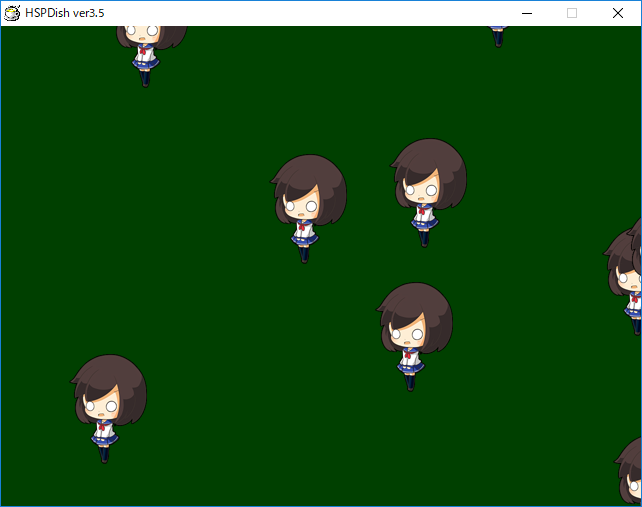
\includegraphics[keepaspectratio,width=8.811cm,height=6.946cm]{text04-img/text04-img036.png}
      \caption{array.hspの実行画面}
    \end{center}
    \label{fig:prog_menu}
\end{figure}

ここでは、10個の絵を同時に動かしています。

最初の絵はx(0)とy(0)、次の絵はx(1)とy(1)…という感じに、変数x,yに番号をつけて複数の絵を管理しています。次のようにrepeat命令とloop命令による繰り返しを使うことで、さらに便利に配列変数を使うことができます。


\begin{description}
    \item \textgt{\bf \ \ repeat 10\ \ \ \ ; 10回繰り返し}
    \item \textgt{\bf \ \ \ \ pos x(cnt),y(cnt)\ \ ; 表示位置を設定する}
    \item \textgt{\bf \ \ \ \ celput 1\ \ \ \ ; 画像を描画する}
    \item \textgt{\bf \ \ loop\ \ \ \ \ \ ; 繰り返し終わり}
\end{description}

repeat〜loop命令で繰り返している間は、システム変数cntが0,1,2…と順番に変化します。これを使って配列の要素を切り替えながら、それぞれの座標に描画することになります。

自分なりにプログラムを改造しながら、どのように変化するか確認してみましょう。

今は10個の絵を動かしていますが、もっと多くするにはどうすればいいか考えてみましょう。

%2369



